\chapter{Background}

\section{Convolutional Neural Networks}

\gls{cnn}s are widely used in image classification tasks, because they look at a collection of spacially connected pixels, and is therefore robust to objects being framed differently. 

\section{Pose Estimation}
In this work we are heavily inspired by \cite{cao2017realtime} that uses two convolutional neural networks to find human pose. One of the networks finds the probability for the 2D location of a set of joints, we get $N$ confidence maps for the locations of each $N$ number of joints. The other creates $M$ \gls{paf} the probability maps for $M$ number of limbs\footnote{In this work we'll stick to the convention of using the term limb to describe any connection between any pair of body landmarks, which we call joints.}. We then use the results from this \gls{paf} to find out which joints from the first result should be connected.

\begin{figure}[h]
  \begin{subfigure}[t]{0.24\textwidth}
    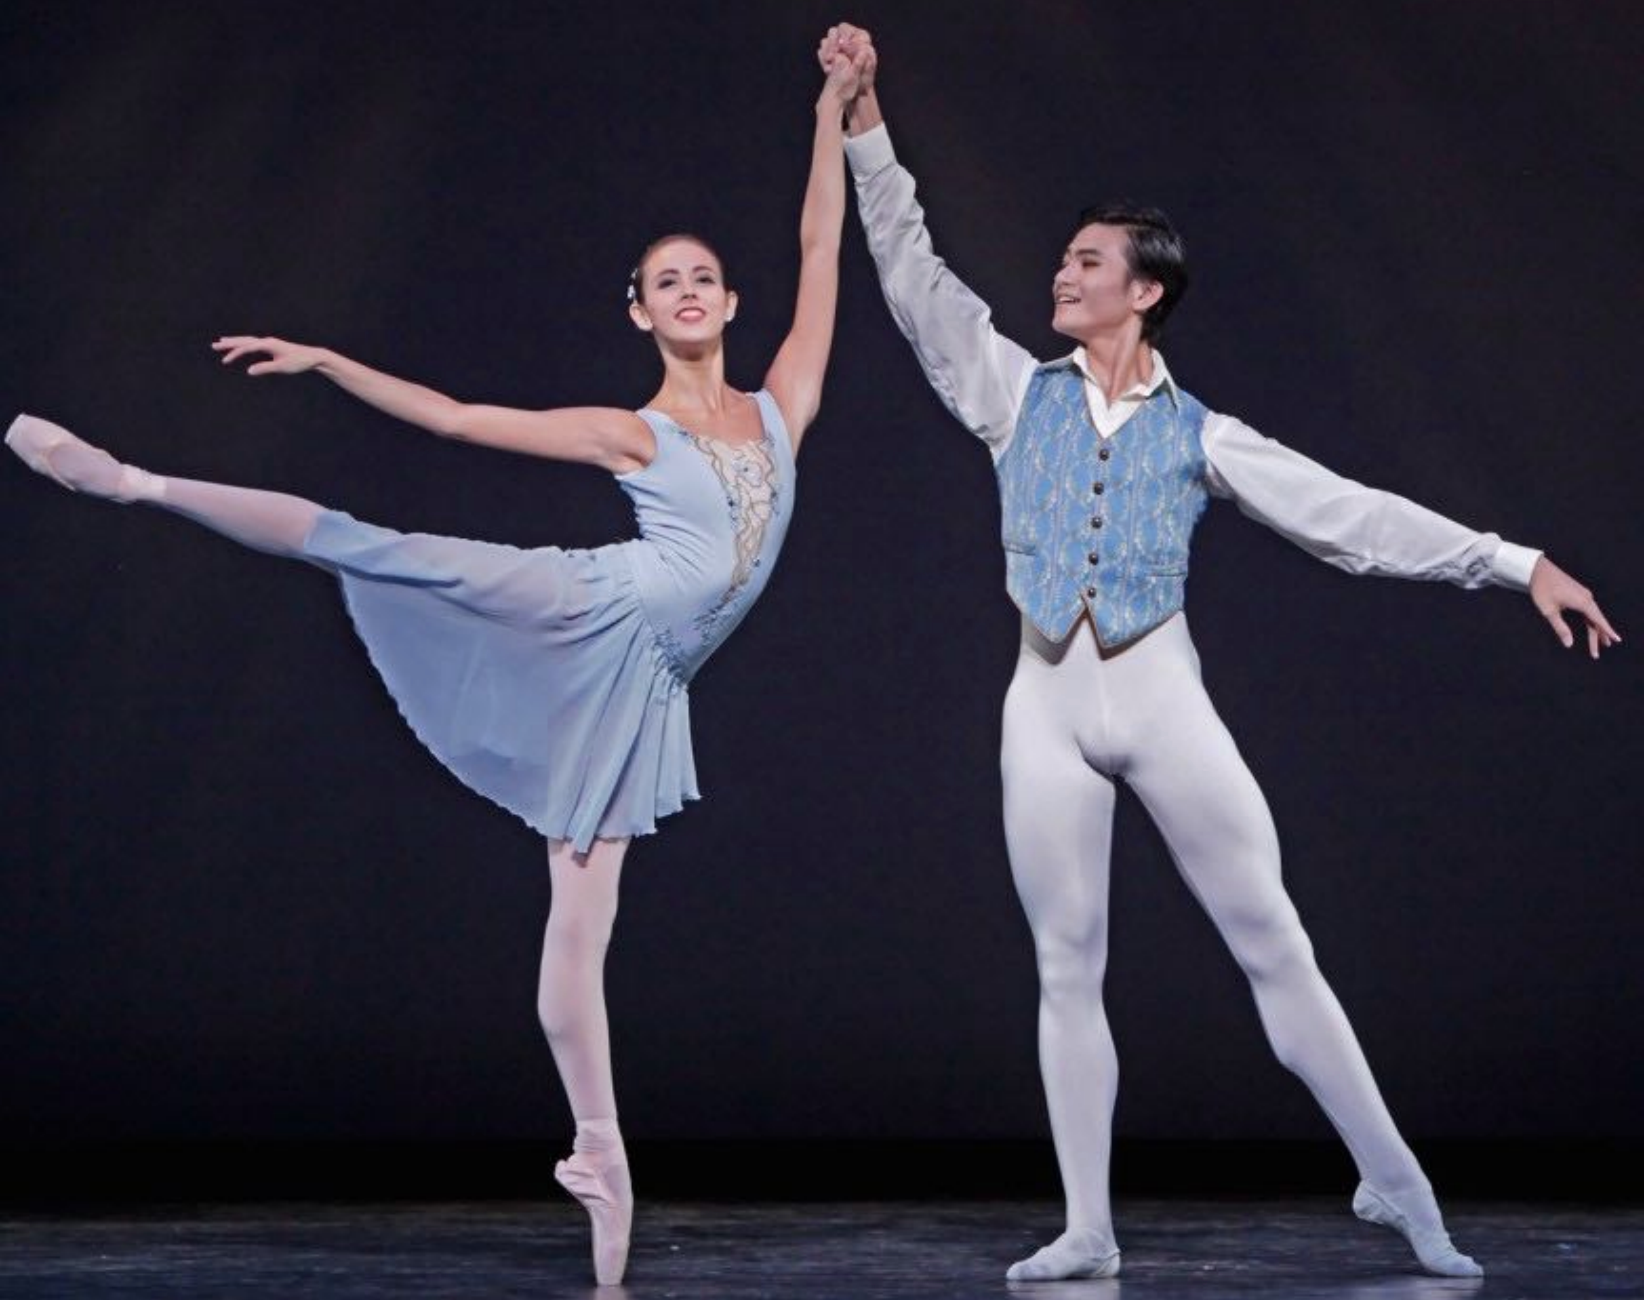
\includegraphics[width=1\linewidth]{img/openpose_pipeline_a}
    \caption{Input Image}
    \label{fig:oppA}
  \end{subfigure}%
  ~
  \begin{subfigure}[b]{0.24\textwidth}
    \begin{subfigure}{1\textwidth}
      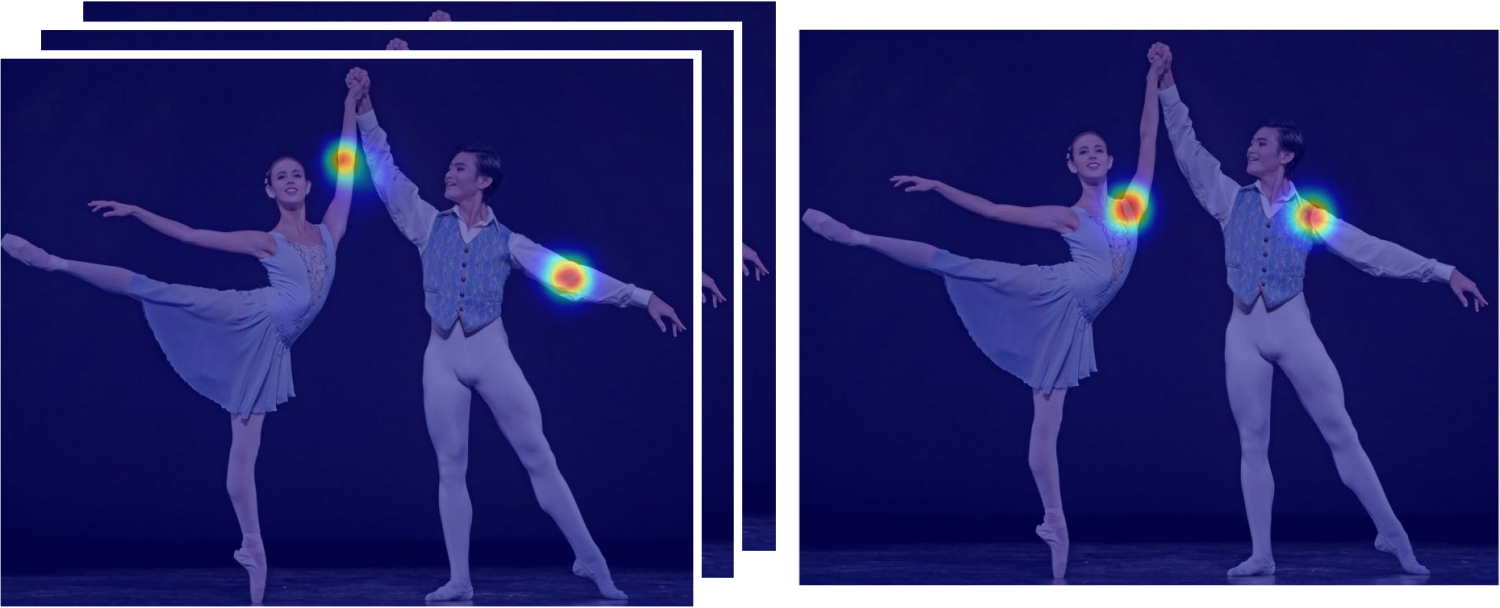
\includegraphics[width=1\linewidth]{img/openpose_pipeline_b}
      \caption{Part Confidence Maps}
      \label{fig:oppB}
    \end{subfigure}
    
    \begin{subfigure}{1\textwidth}
      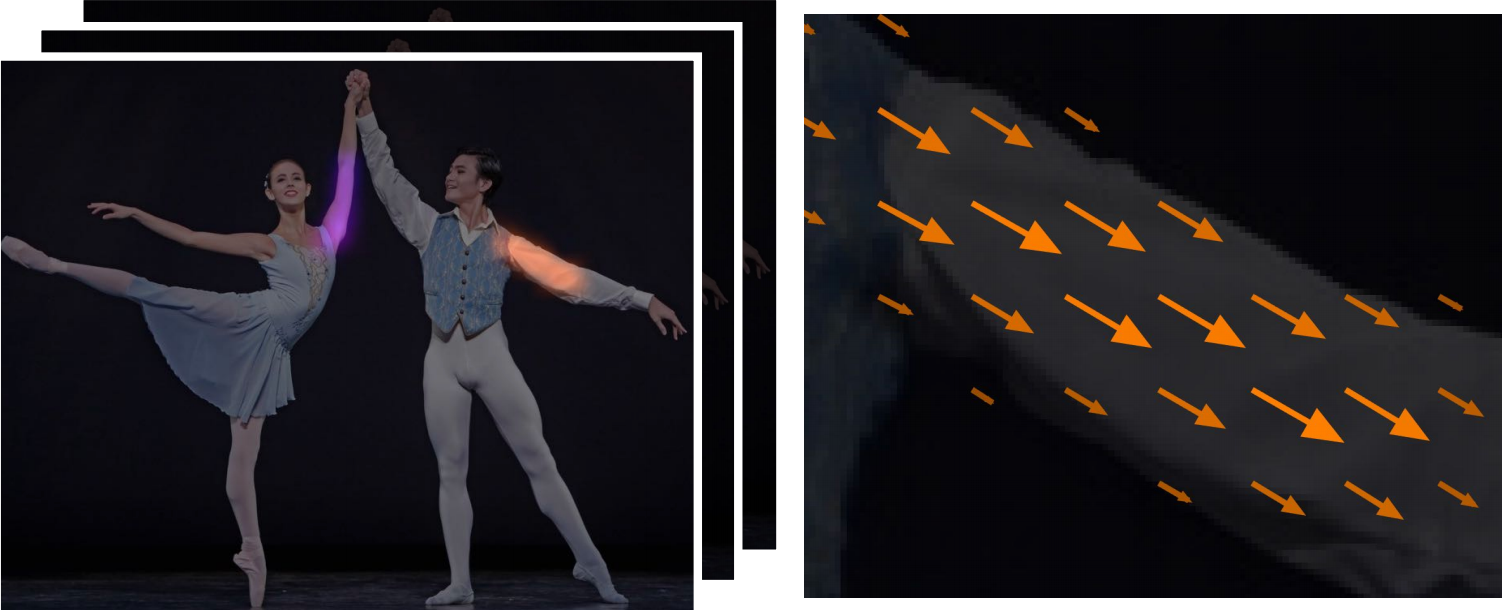
\includegraphics[width=1\linewidth]{img/openpose_pipeline_c}
      \caption{Part Affinity Fields}
      \label{fig:oppC}
    \end{subfigure}
  \end{subfigure}%
  ~
  \begin{subfigure}[t]{0.24\textwidth}
    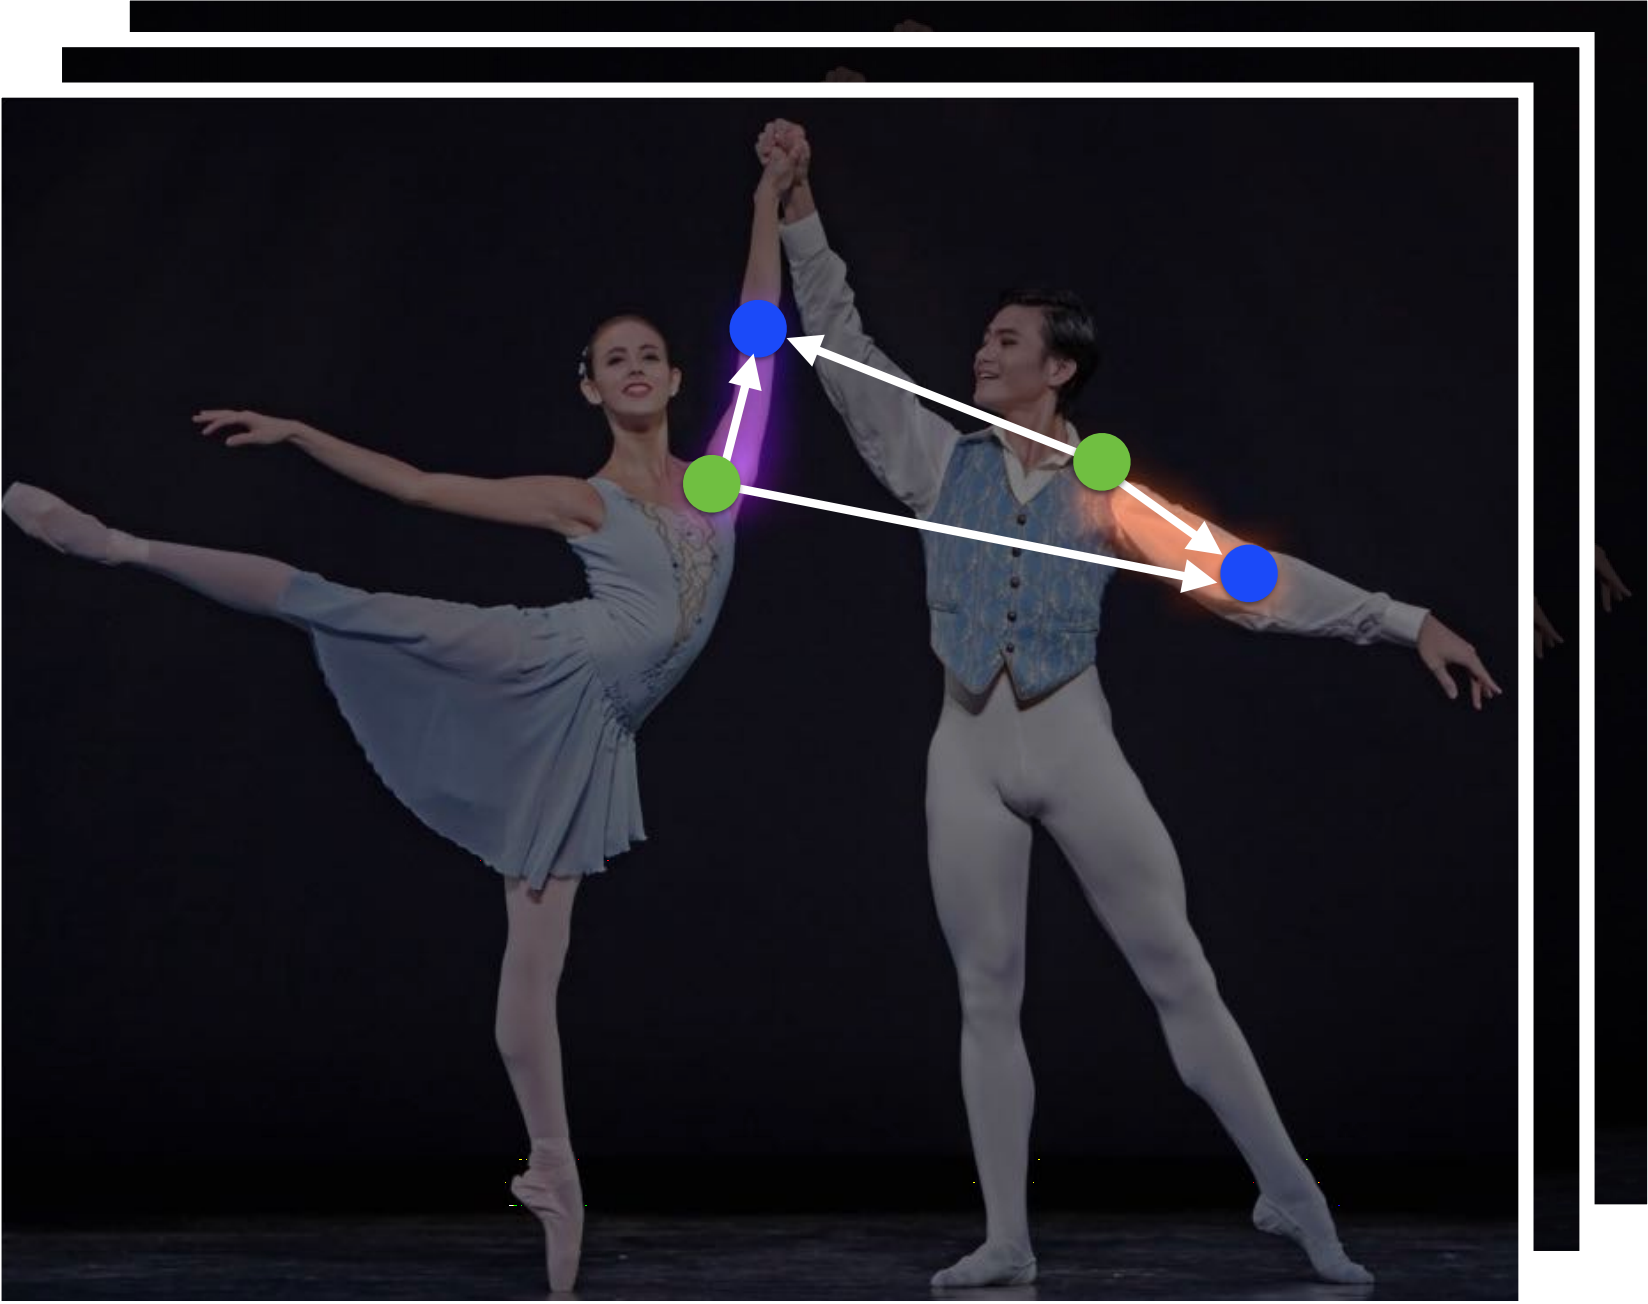
\includegraphics[width=1\linewidth]{img/openpose_pipeline_d}
    \caption{Bipartite Matching}
    \label{fig:oppD}
  \end{subfigure}%
  ~
  \begin{subfigure}[t]{0.24\textwidth}
    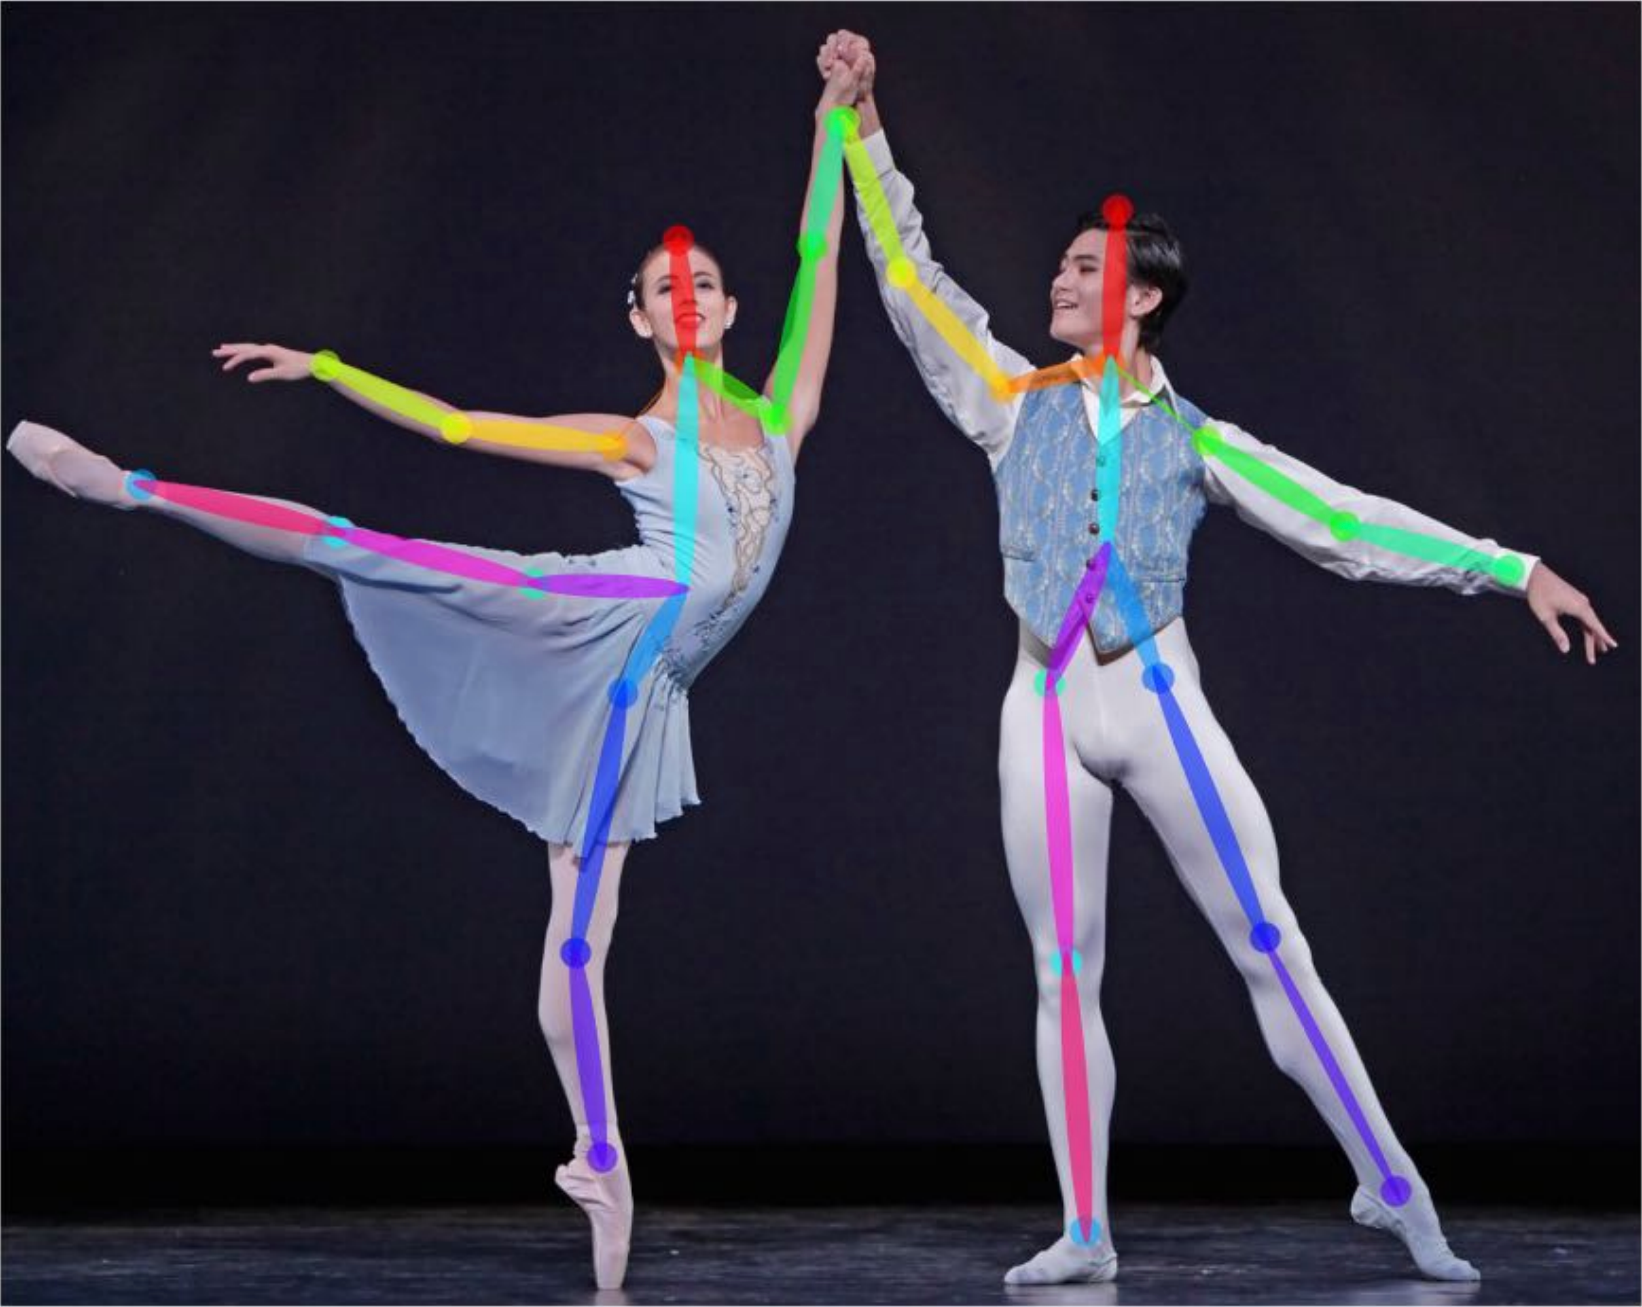
\includegraphics[width=1\linewidth]{img/openpose_pipeline_e}
    \caption{Parsing Results}
    \label{fig:oppE}
  \end{subfigure}
  \caption[OpenPose pipeline]{The pipeline described in \cite{cao2017realtime}. The input image
    \ref{fig:oppA} is fed into the two networks which produce joint detections in
    confidence maps \ref{fig:oppB} and \gls{paf}s \ref{fig:oppC}. They then preform
    bipartite matching in \ref{fig:oppD} to determine which detected joints should be
    connected by a limb. \ref{fig:oppE} shows the finished results.}
  \label{fig:openpose_pipeline}
\end{figure}

Using the method described in \cite{cao2017realtime} we however don't get any information if some pairs of joints are missing, for example due to occlusion or failure to detect the body landmark, leading to an incomplete skeleton.


A lot of research\footnote{TODO: Cite Research} has been going into extracting human pose either from RGB images, or using depth images. Although many methods exists such as \emph{Histogram of Gradients (HoG)} classifiers,

A lot of research has been done in estimating human pose in two dimensions, as this is where we have quite large datasets, such as the MPII, or the Human 3.6M datasets \cite{andriluka14cvpr,h36m_pami}.


